\documentclass{article}

% Language setting
% Replace `english' with e.g. `spanish' to change the document language
\usepackage[english]{babel}
\usepackage{float}

% Set page size and margins
% Replace `letterpaper' with `a4paper' for UK/EU standard size
\usepackage[letterpaper,top=2cm,bottom=2cm,left=3cm,right=3cm,marginparwidth=1.75cm]{geometry}

% Useful packages
\usepackage{amsmath}
\usepackage{graphicx}
\usepackage[colorlinks=true, allcolors=blue]{hyperref}

\title{Pattern Recognition \\\Large{Exercise 2}}
\author{Tobias Verheijen, Mattéo Bonvin, Zhihui Wang}
\date{}

\begin{document}
\maketitle

\section{SVM}
For the SVM, we used Sklearn's svm.SVC. This was easy to implement, but without adjusting certain parameters our dataset was too large for the model to run within a reasonable amount of time (e.g. over 6 hours of computation on 16 CPU cores without a result). Once we found the \textit{maxiters} parameter it was much more manageable to run. With a \textit{maxiters} value of 500, we reduced run-time to around 35 minutes per core.
The results of the Cross Validation are as follows:

\begin{table}[H]
\centering
\begin{tabular}{l|c|r}
CV idx & C Value & Score \\\hline
1 & 0.1 & 0.834 \\
1 & 1 & 0.822 \\
1 & 10 & 0.822 \\
1 & 100 & 0.822 \\
2 & 0.1 & 0.837 \\
2 & 1 & 0.815 \\
2 & 10 & 0.815 \\
2 & 100 & 0.815 \\
3 & 0.1 & 0.829 \\
3 & 1 & 0.816 \\
3 & 10 & 0.816 \\
3 & 100 & 0.816 \\
\end{tabular}
\caption{Linear SVM Cross-Validation}
\end{table}

\begin{table}[H]
\centering
\begin{tabular}{l|c|r}
CV idx & C Value & Score \\\hline
1 & 0.1 & 0.891 \\
1 & 1 & 0.960 \\
1 & 10 & 0.967 \\
1 & 100 & 0.967 \\
2 & 0.1 & 0.888 \\
2 & 1 & 0.956 \\
2 & 10 & 0.966 \\
2 & 100 & 0.965 \\
3 & 0.1 & 0.887 \\
3 & 1 & 0.959 \\
3 & 10 & 0.965 \\
3 & 100 & 0.965 \\
\end{tabular}
\caption{RBF SVM Cross-Validation}
\end{table}

The accuracy on the test set was:
\begin{table}[H]
\centering
\begin{tabular}{l|c|r}
Kernel & C Value & Accuracy \\\hline
Linear & 0.1 & 0.7981 \\
RBF & 1 & 0.9691 \\
\end{tabular}
\caption{SVM Test Set accuracy}
\end{table}

\section{MLP}

For the MLP, we used PyTorch. We tried first with other librairies but the process would take too much time. With \textit{torch}, the process takes about 30 minutes to find a result.
The Epoch result is the following : 
\begin{table}[h]
    \centering
    \begin{tabular}{|c|c|c|}
        \hline
        Epoch & Train Loss & Validation Loss\\
        \hline
        1/10 & 0.5429 & 0.1659 \\
        2/10 & 0.1832 & 0.1409 \\
        3/10 & 0.1572 & 0.1336 \\
        4/10 & 0.1515 & 0.1420 \\
        5/10 & 0.1424 & 0.1200 \\
        6/10 & 0.1372 & 0.1302 \\
        7/10 & 0.1334 & 0.1420 \\
        8/10 & 0.1287 & 0.1192 \\
        9/10 & 0.1246 & 0.1001 \\
        10/10 & 0.1259 & 0.1032 \\
        \hline
    \end{tabular}
    \caption{Evolution of Train and Validation Loss}
    \label{tab:Loss}
\end{table}

For an accuracy of 96.05\%

Here is the graph generated : 
\begin{figure}[h]
    \centering
    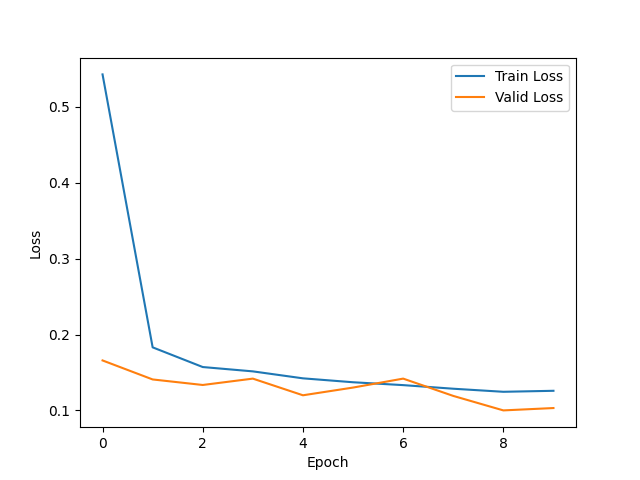
\includegraphics[width=0.5\textwidth]{Figures/MLP_TrainLoss_ValidLoss.png}
    \caption{Train and Valid Loss of the MLP}
    \label{fig:TrainValidLoss_MLP}
\end{figure}

\end{document}
